\documentclass[../master]{subfiles}

\begin{document}

\chapter{MAIKo TPC}
\section{MAIKo TPC とは}
Time Projection Chamber (TPC) は荷電粒子のトラックを検出するために広く用いられている検出器である.
荷電粒子がTPC の検出ガス中を通過するとき,飛跡の周囲の粒子をイオン化させる.
イオン化で発生した電子をドリフト電場 (図\ref{fig::MAIKo_view}中$y$軸方向) により
読み出し面にドリフトさせることでトラックを検出する.
図\ref{fig::MAIKo_view}のようにTPC の有感領域中で入射粒子と標的粒子を反応させることで,
散乱点の周りを有感領域で覆うことができる.
そのため,散乱で放出される低エネルギーの荷電粒子を大立体角で検出することができる.
このような検出器としてMAIKo TPC が開発された.
MAIKo TPC の写真を図\ref{pic::MAIKo}に示す.
\begin{figure}
  \centering
  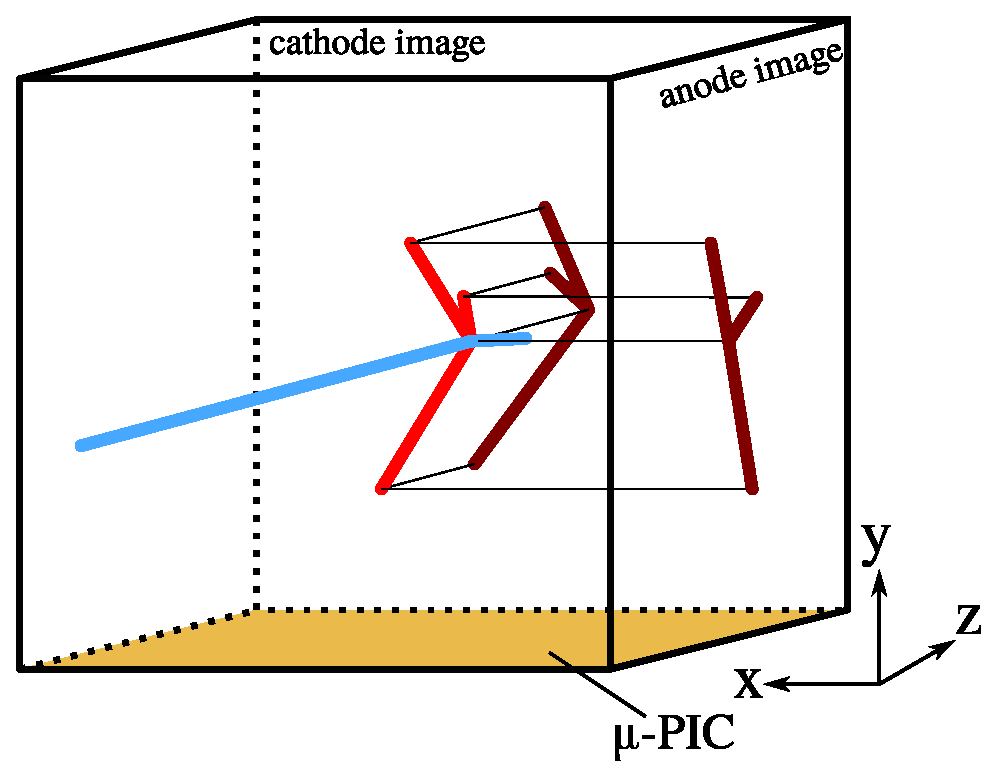
\includegraphics[clip, width=0.7\columnwidth]{MAIKo2.eps}
  \caption[MAIKo TPC の概観図.]{MAIKo TPC の概観図.
    図では紙面手前から入射した中性子 (青) がTPCの中の${}^{12}{\rm C}$と散乱して3つの$\alpha$粒子 (赤) に崩壊した事象を表す.
    anode image ($zy$平面) と cathode image ($zy$平面) の2平面に荷電粒子のトラックが射影される.
    中性子は電荷を持たないためanode \& cathode image にトラックとして検出されない.
  }
  \label{fig::MAIKo_view}
\end{figure}
\begin{figure}
  \centering
%  \includegraphics[clip, width=0.7\columnwidth]{}
  \caption[MAIKo TPC の概観.]{MAIKo TPC の概観.}
  \label{pic::MAIKo}
\end{figure}

\subsection{MAIKo TPC の構造}
\label{sec::maiko-cage}
図\ref{fig::MAIKo_cage}にMAIKo TPC の構造を示す.
\begin{figure}
  \centering
  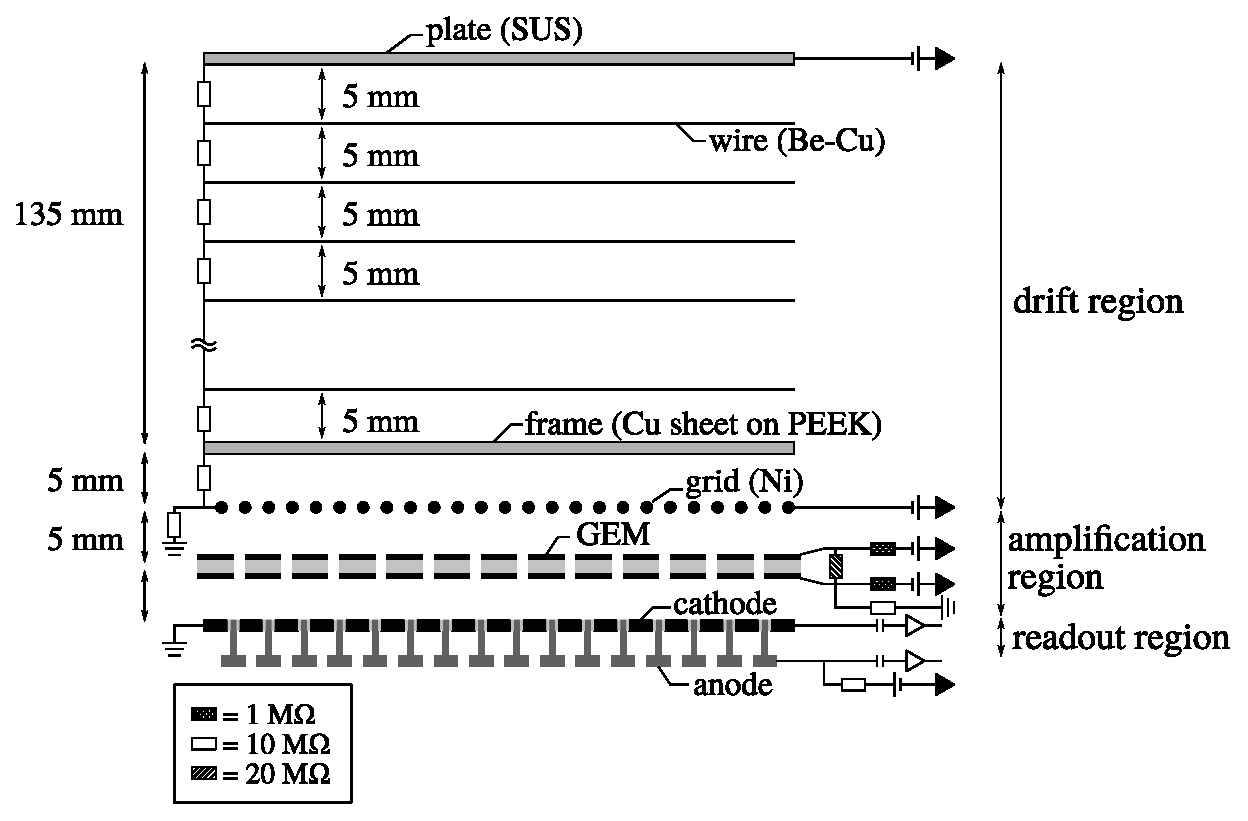
\includegraphics[clip, width=\columnwidth]{MAIKo_cage.eps}
  \caption{MAIKo TPC の構造.}
  \label{fig::MAIKo_cage}
\end{figure}
MAIKo TPC はplate,wire,grid,GEM (gas electron multiplier),$\mu$-PICからなる.
plate,grid,GEM,$\mu$-PICにHV が接続されている.
plate,wire,girdの間は\SI{10}{\mega\ohm}の抵抗で繋がれている.
GEM とHV は\SI{1}{\mega\ohm}と\SI{20}{\mega\ohm}の抵抗で繋がれている.
plateからgridの間の領域をドリフト領域,
gridから$\mu$-PICの間の領域を増幅領域,
$\mu$-PICの周囲を読み出し領域と呼ぶ.

%plate とgrid に電圧をかけることでドリフト領域にドリフト電場を形成する.
%ドリフト領域を荷電粒子が通過する際に生成された電子がドリフト電場によって増幅領域へ移動する.
%ドリフト電場を一様に形成するために5 mm間隔でドリフト領域の周囲にwire を巻いてある.
%ドリフト領域はドリフト方向に140 mm である.
%ドリフトしてきた電子は,まずGEM (gas electron multiplier) で増幅される.
%増幅した電子およびイオンによって$\mu$-PIC のanode とcathode に誘起された信号を読み出す.
%$\mu$-PIC では信号の読み出しだけでなく電子の増幅も行われる.

\subsection{ドリフト領域}
grid からplate の方向 (図\ref{fig::MAIKo_cage}では上向き) にドリフト電場を作ることで
トラックの周りに発生した電子を増幅領域へドリフトさせる.
ドリフト電場の一様性が高いほど,電子を均等にドリフトすることができる.
ドリフト電場を一様に形成するためにwire が\SI{5}{\milli\metre}間隔で巻かれている~\cite{furuno}.
ドリフト領域はドリフト電場の方向に\SI{140}{\milli\metre}である.
この領域がMAIKo TPC の有感領域となる.

\subsection{増幅領域}
MAIKo TPC ではGEM と$\mu$-PICを用いて電子の増幅を行う.
GEM は,図\ref{pic::GEM}のようにポリマーのフィルムの表面を銅で被覆し,
直径\SI{70}{\micro\metre} の穴を\SI{140}{\micro\metre}間隔で\SI{1}{\square\milli\metre}あたり
100 個の密度で開けたものである.
銅の2つの層はポリマーによって絶縁されている.
銅の両面に電圧を印加することによって,高電場が形成されドリフトしてきた電子が増幅される.
\begin{figure}
  \centering
  %\includegraphics[clip, width=0.7\colmunwidth]{}
  \caption{GEM の拡大図.}
  \label{pic::GEM}  
\end{figure}
\begin{figure}
  \centering
  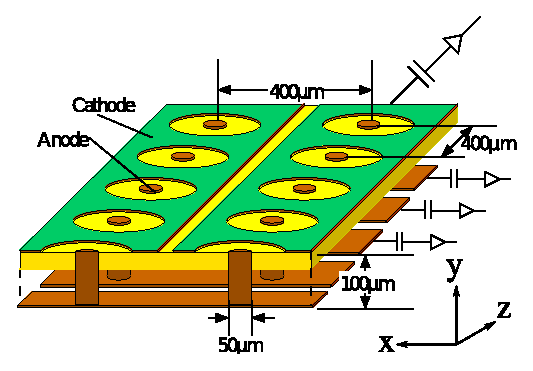
\includegraphics[clip, width=0.7\columnwidth]{upic_struc_xyz.eps}
  \caption[$\mu$-PICの概観図.]{$\mu$-PICの概観図.
    図中の横方向にanode strip,奥行き方向にcathode strip が配置されている.
  }
  \label{fig::mupic}
\end{figure}
$\mu$-PIC は図\ref{fig::mupic}のようにanode strip とcathode strip が直交するように配置されている.
anode strip,cathode strip ともに\SI{400}{\micro\metre}間隔でそれぞれ256~ch分割されている.
直径\SI{50}{\micro\metre}の円柱状のanode 電極に高電圧をかけることで高電場を形成することができ,
$\mu$-PICによって信号が読み出される直前に電子が増幅される.

\subsection{読み出し領域}
\label{sec::mu-pic}
図\ref{fig::MAIKo_view}中でanode strip は$z$軸,cathode strip は$x$軸と平行になるように$\mu$-PICが配置されている.
ドリフト電場により移動してきた電子をanode strip,cathode strip により読み出し,
それぞれ$x$軸,$z$軸座標を検出することができる.
また,anode strip,cathode strip で検出される信号の時間分布により$y$軸座標を決定することができる.

MAIKo TPC からは図\ref{fig::track_demo}のようにトラックが
anode strip に垂直な面 ($z-y$平面) に射影されたanode image と
cathode strip に垂直な面 ($z-y$平面) に射影されたcathode image の2つの画像が出力される.
anode strip とcathode strip はそれぞれ256~chで構成され,
読み出される信号波高の時間変化は\SI{100}{\mega\hertz}で1,024~samples測定されるため,
出力される画像の解像度は$256\times1,014$~pixels となる.
\begin{figure}
  \centering
  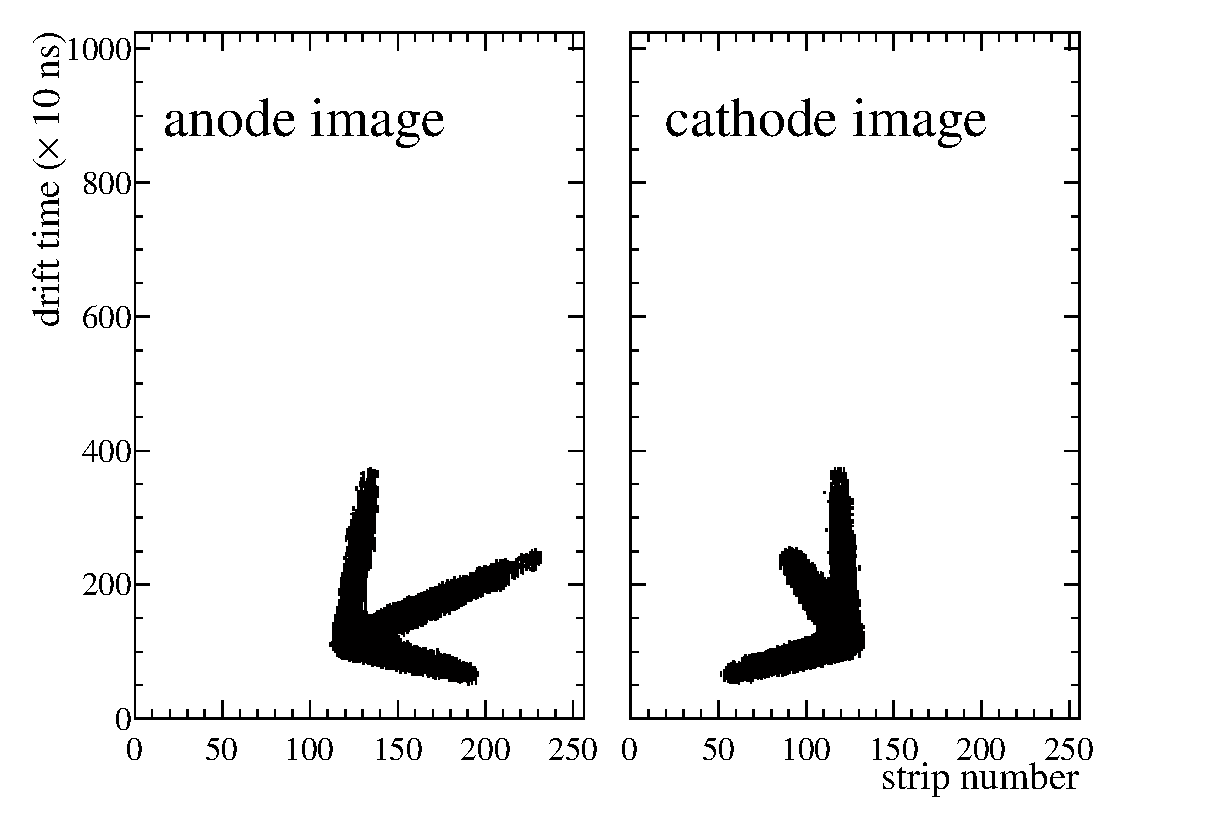
\includegraphics[clip, width=0.9\columnwidth]{10024_4.eps}
  \caption[MAIKo TPC から得られず画像データの一例.]
          {MAIKo TPC から得られず画像データの一例.
          このイベントは\ref{chap::simulation}章で述べるシミュレーションによって生成したデータである.}
  \label{fig::track_demo}
\end{figure}
また,anode strip,cathode strip ともに32~chごとにまとめて信号をFADC で波形を取得している.
FADC で取得した信号の一例を図\ref{fig::FADC_waveform}に示す.
FADC では\SI{25}{\mega\hertz}で信号波形を取得される.
\begin{figure}
  \centering
  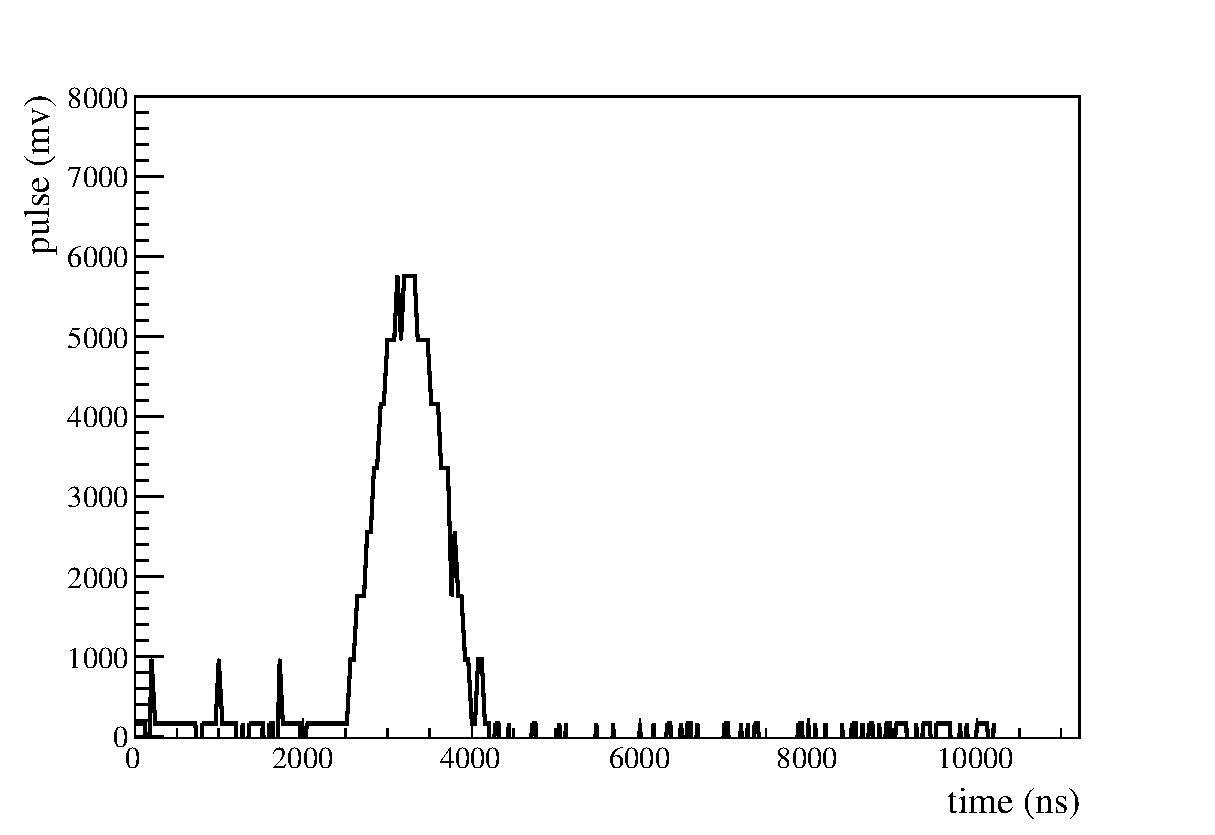
\includegraphics[clip, width=0.7\columnwidth]{0101_waveform_8.eps}
  \caption{FADCで取得された$\mu$-PICの信号波形の一例.}
  \label{fig::FADC_waveform}
\end{figure}

\section{検出ガスの候補}
\label{sec::detection_gas_candidate}
標的に${}^{12}{\rm C}$を用いるため分子中に炭素を含むガスを検出ガスに用いる.
${}^{12}{\rm C}$以外の原子核が含まれるガスを用いると背景事象となるため,
水素と炭素以外の原子が含まれない炭化水素を用いる.
陽子,${}^{4}{\rm He}$と14 MeV の中性子の散乱は複数の荷電粒子に崩壊しないため,
トラックの本数から背景事象を取り除くことができる.
炭化水素の代表的なガスは,メタン (\Methane) やエタン (${\rm C_{2}H_{6}}$),
イソブタン (\isoButane) である.
また,水素ガスやヘリウムガスとの混合ガスも用いることができる.
検出ガスとして求められる性能には以下のようなものがある.
\begin{itemize}
\item
  放電しにくい
\item
  荷電粒子のエネルギー損失 ($dE/dx$) が適切である
\item
  ${}^{12}{\rm C}$の量が少なくない
\item
  適切なドリフト速度を達成できる
\item
  適切なドリフト電場のもとでディフュージョンが小さい
\end{itemize}
これらの項目を基準に検出ガスの種類と圧力の決定を行う.

\subsection{エネルギー損失}
荷電粒子のエネルギー損失 ($dE/dx$) が大きくなりすぎるとガス中での飛行距離が短くなり,
トラックとして認識することが難しくなる.
本実験では荷電粒子のエネルギーをトラックの長さから決定する.
そのため,$dE/dx$ が小さくなりすぎるとトラックが有感領域で止まらず,
トラックの長さ (エネルギー) を決定することができなくなる.
検出する対象である$\alpha$粒子の $dE/dx$ が適切な大きさとなるガスの種類と圧力の候補を選出する.

まず,代表的な炭化水素である\Methane を考える.
ガス中で\SI{15}{\milli\metre} 以上飛行し,MAIKo TPC の有感領域中で停止する$\alpha$粒子を検出可能な$\alpha$粒子と定義する.
図\ref{fig::alpha_E_dist}に示したエネルギー分布の$\alpha$粒子のうち,
検出できた割合の圧力依存性を図\ref{fig::efficiency_P_dist}に示す.
このとき,散乱点がビーム軸上に一様に分布しているとして計算した.
図\ref{fig::efficiency_P_dist}から分かるように,\SI{50}{\hecto\pascal} で最大となっている.
\begin{figure}
  \centering
  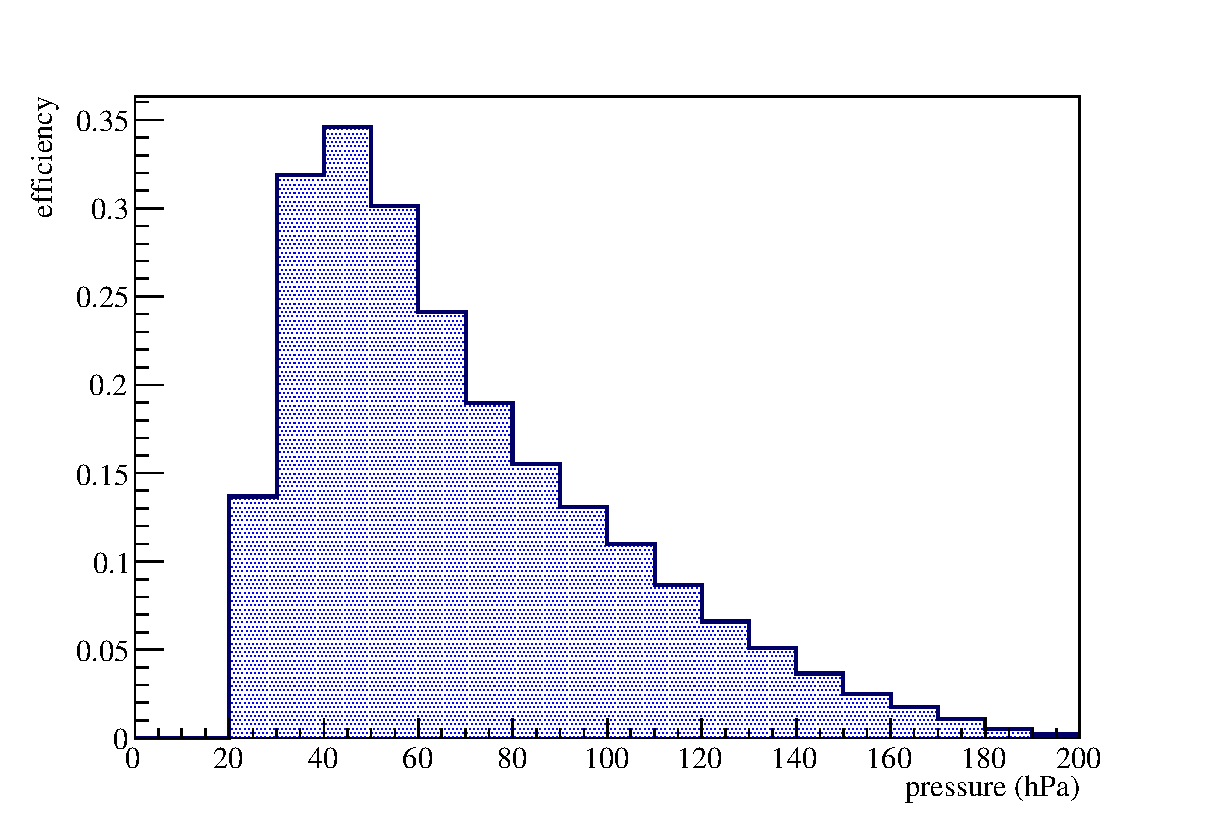
\includegraphics[clip, width=0.7\columnwidth]{efficiency_P_dist.eps}
  \caption[\Methane の圧力による検出効率の分布.]
          {\Methane の圧力による検出効率の分布.
            $\alpha$粒子は図\ref{fig::alpha_E_dist}に示したエネルギー分布を仮定した.
           }
  \label{fig::efficiency_P_dist}
\end{figure}
\SI{50}{\hecto\pascal}のときの\Methane の各種の値は表\ref{tab::CH4_50_params}のとおりである.
\begin{table}
  \centering
  \caption{\SI{50}{\hecto\pascal}のときの\Methane のパラメータ.}
  \label{tab::CH4_50_params}
  \begin{tabular}{cc}
    \toprule
    項目 & 値\\
    \midrule
    密度 & \SI{3.29e-5}{\gram\per\cubic\centi\metre} \\
    $dE/dx$ ($E_{\alpha} = \SI{0.5}{\mega\electronvolt}$, \SI{10}{\milli\metre}) & \SI{0.107}{\mega\electronvolt}\\
    飛距離 ($E_{\alpha} = \SI{0.5}{\mega\electronvolt}$) & \SI{65.6}{\milli\metre} \\
    \bottomrule
  \end{tabular}
\end{table}

\SI{50}{\hecto\pascal}のときの\Methane の$dE/dx$と同程度となる,他のガスを考えていく.
表\ref{tab::mixture}に示した6つを候補とした.
混合ガスでは圧力を\SI{100}{\hecto\pascal} に固定し混合比をパラメータとして$dE/dx$を合わせる.
括弧内はガスの混合の割合を示す.
\begin{table}
  \centering
  \caption[ガスの混合パターン,圧力,$dE/dx$.]
          {ガスの混合パターン,圧力,$dE/dx$.
          括弧内はガスの混合の割合を示す.}
  \label{tab::mixture}
  \begin{tabular}{ccccc}
    \toprule
    gas &
    \begin{tabular}{c}
      pressure \\
      (\si{\hecto\pascal})
    \end{tabular} &
    \begin{tabular}{c}
      density \\
      (\si{\gram\per\cubic\centi\metre})
    \end{tabular} &
    \begin{tabular}{c}
      $dE/dx$ (\si{\mega\electronvolt})\\
      $E_{\alpha} = \SI{0.5}{\mega\electronvolt}$ \\
      \SI{10}{\milli\metre}
    \end{tabular} &
    \begin{tabular}{c}
      ドリフト電場 (\si{\volt\per\milli\metre}) \\
      @ \SI{0.014}{\milli\metre\per\nano\second}
    \end{tabular}\\
    \midrule
    \Methane         & 50  & 3.29$\times 10^{-5}$ & 0.107 & 0.418 \\
    \MethaneHydro    & 100 & 2.55$\times 10^{-5}$ & 0.107 & 4.31 \\
    \MethaneHerium   & 100 & 3.62$\times 10^{-5}$ & 0.109 & 1.89 \\
    \isoButane       & 15  & 3.58$\times 10^{-5}$ & 0.102 & 0.644 \\
    \isoButaneHydro  & 100 & 3.13$\times 10^{-5}$ & 0.122 & 6.80 \\
    \isoButaneHerium & 100 & 3.86$\times 10^{-5}$ & 0.102 & 3.26 \\
    \bottomrule
  \end{tabular}
\end{table}
これらの6種類の候補から検出ガスを選ぶ.

\subsection{ドリフトスピード}
MAIKo TPC では\SI{100}{\mega\hertz}で1024 samples データを取得するため,
ドリフト方向は\SI{10.24}{\micro\second}のタイムウィンドウが開いている.
ドリフトケージの大きさ (\SI{140}{\milli\metre}) を可能な限りタイムウィンドウに収めるためには,\si{\micro\second}
ドリフトスピードを$\SI{140}{\milli\metre}/\SI{10.24}{\micro\second} \sim \SI{0.014}{\milli\metre\per\nano\second}$
に調整する必要がある.
Magboltz~\cite{magboltz} によって計算したドリフト電場とドリフトスピードの関係を図\ref{fig::drift_v_magboltz}に,
ドリフトスピードが\SI{0.014}{\milli\metre\per\nano\second}となるドリフト電場の値を表\ref{tab::mixture}に示す.
図\ref{fig::drift_v_magboltz}の横方向の点線は\SI{0.014}{\milli\metre\per\nano\second}を表す.
以降,これらのドリフト電場で評価を行う.
\begin{figure}
  \centering
  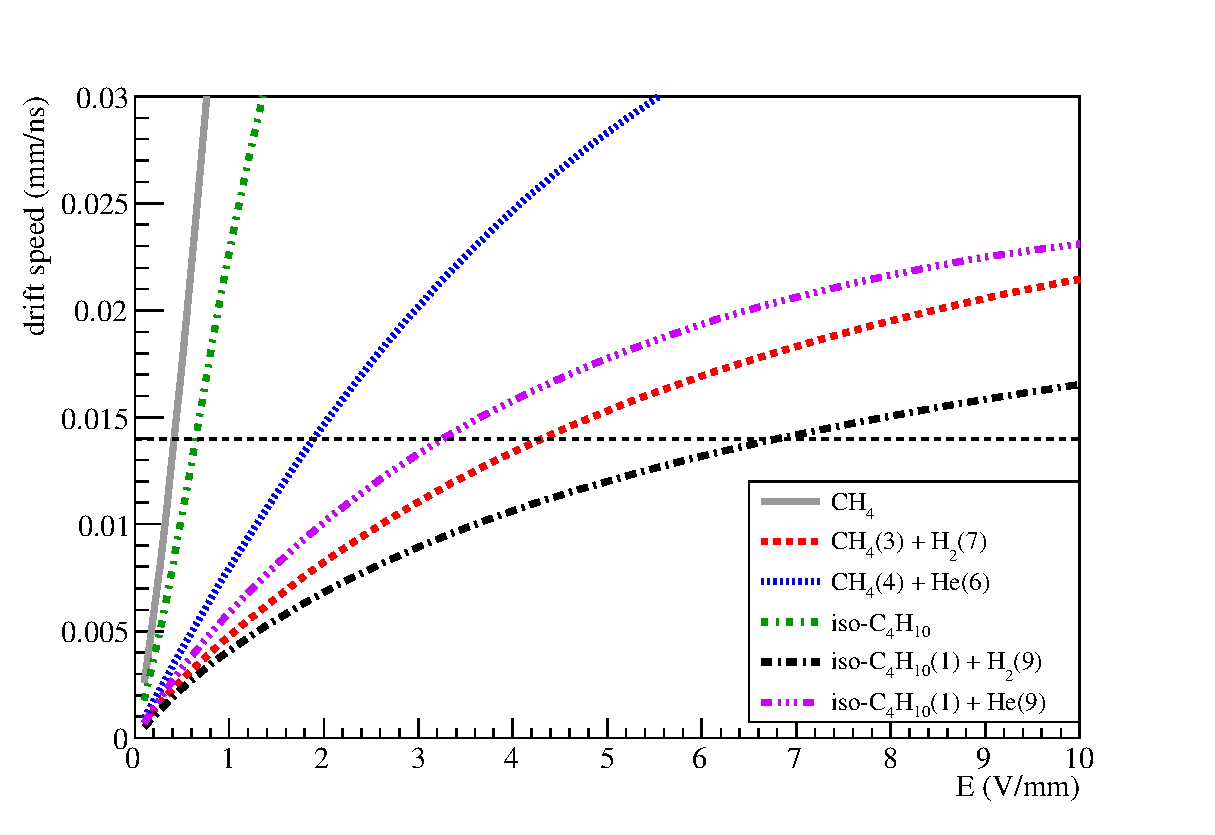
\includegraphics[clip, width=0.9\columnwidth]{drift_v_magboltz.eps}
  \caption[ドリフト電場とドリフトスピードの関係.]
          {ドリフト電場とドリフトスピードの関係.
            \Methane は\SI{50}{\hecto\pascal},\isoButane は\SI{15}{\hecto\pascal},その他は\SI{100}{\hecto\pascal}である.
          横方向の点線は\SI{0.014}{\milli\metre\per\nano\second}を示す.}
  \label{fig::drift_v_magboltz}
\end{figure}

\subsection{ディフュージョン}
ドリフト電場によって電子が移動する間に検出ガスとの散乱と電子の熱運動により,
図\ref{fig::diffusion-image}のように広がりながらドリフトする.
\begin{figure}
  \centering
  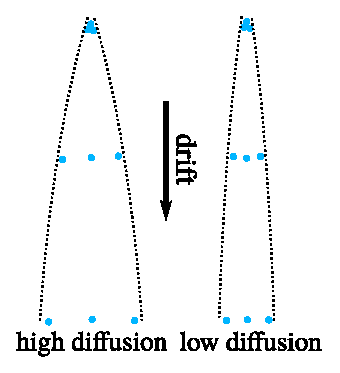
\includegraphics[clip, width=0.4\columnwidth]{diffusion_image.eps}
  \caption[ディフュージョンによって電子が拡散するイメージ.]
          {ディフュージョンによって電子が拡散するイメージ.
          同じ位置で生成された電子でもドリフトする間に位置が拡散する.}
  \label{fig::diffusion-image}
\end{figure}
電子が広がることをディフュージョンと呼ぶ.
この効果が大きくなると,
荷電粒子によって同じ場所に生成された電子が$\mu$-PICに到達するまでに広がるため,
トラックが太く検出される.
トラックが太くなると,複数のトラックを分離することが難しくなる.
そのため,ディフュージョンの効果が小さいことが望まれる.

ドリフト電場がない場合のディフュージョンは以下のように理解できる.
電子は熱運動により発生点から拡散する.
熱運動の平均速度$v$はMaxwell 分布により
\begin{equation}
  v = \sqrt{\frac{8k_{B}T}{\pi m}}
  \label{eq::maxwell_velocity}
\end{equation}
と表せる.
ここで$k_{B}$はボルツマン定数,$T$は温度,$m$は粒子の質量である.
電子が発生した時刻から$\Delta t$後では,
\begin{equation}
  \frac{N_0}{\sqrt{4\pi D t}}\exp\left(-\frac{x^{2}}{4 D t}\right)
  \label{eq::gaus_dist}
\end{equation}
のガウス分布で電子が広がる.
ここで$N_{0}$は全粒子数,$x$は発生した点からの距離,$D$はディフュージョン係数を表す.
ディフュージョン係数$D$は電子の平均自由工程$\lambda$を用いて
\begin{equation}
  D = \frac{1}{3}v\lambda
  \label{eq::diffusion_coef}
\end{equation}
と表せる.
理想気体において平均自由工程$\lambda$は,ガスとの散乱の全断面積$\sigma_{0}$,圧力$p$のもとで
\begin{equation}
  \lambda = \frac{1}{\sqrt{2}}\frac{k_{B}T}{\sigma_{0}p}
  \label{eq::lambda}
\end{equation}
と表される.
式\ref{eq::maxwell_velocity}, \ref{eq::diffusion_coef}, \ref{eq::lambda}により,
\begin{equation}
  D = \frac{2}{3\sqrt{\pi}}\frac{1}{p\sigma_{0}}\sqrt{\frac{\left(k_{B}T\right)^{3}}{m}}
  \label{eq::diffusion_coef_2}
\end{equation}
となる.
式\ref{eq::diffusion_coef_2}より,
同じガスでは圧力が高いほど,温度が低いほどディフュージョン係数が小さいことが分かる.

ドリフト電場がある場合,発生点からの距離を$L$,ドリフトスピードを$drift\_v$とすると,
\begin{equation}
  \Delta t = \frac{L}{drift\_v}
  \label{eq::delta_t}
\end{equation}
となる.
直感的には,式\ref{eq::gaus_dist}の分散$\sigma(L)$は
\begin{align}
  \sigma(L) & = \sqrt{2 D \Delta t}\\
  & = \sqrt{\frac{2 D}{drift\_v}}\times\sqrt{L}\\
  & = D_{\rm Magboltz}\times\sqrt{L}
\end{align}
となる.
Magboltz によってディフュージョン係数$D_{\rm Magboltz}$が得られる.
Magboltz によって計算したディフュージョン係数を表\ref{tab::diffusion}に示す.
表\ref{tab::diffusion}中の$D_{t}$はドリフト方向に対して垂直な方向への拡散,$D_{l}$は電子の運動方向への拡散の係数を表す.
\begin{table}
  \centering
  \caption[Magboltz で計算したディフュージョンの係数.]
          {Magboltz で計算したディフュージョンの係数.
            ディフージョンの大きさはドリフト電場に依存するため,
            ここではドリフトスピードが0.014 mm/ns になるドリフト電場での値を示す.
          $D_{t}$,$D_{l}$はそれぞれ運動方向に垂直,平行方向のディフュージョン.}
  \label{tab::diffusion}
  \begin{tabular}{cccc}
    \toprule
    gas & $D_{t}~(\sqrt{\si{mm}})$ & $D_{l}~(\sqrt{\si{mm}})$ & ドリフト電場 (\si{\volt\per\milli\metre}) \\
    \midrule
    \Methane & 0.433 & 0.547 & 0.418\\
    \MethaneHydro & 0.214 & 0.171 & 4.31\\
    \MethaneHerium & 0.270  & 0.248 & 1.89\\
    \isoButane & 0.357 & 0.414 & 0.644\\
    \isoButaneHydro & 0.196 & 0.145 & 6.80\\
    \isoButaneHerium & 0.246 & 0.197 & 3.26\\
    \bottomrule
  \end{tabular}
\end{table}
\Methane および\isoButane の単体ではディフージョン係数が大きく,
同じドリフトスピードのとき,ドリフト電場が大きいほどディフュージョン係数が小さいことが分かる.

\isoButaneHydro が最もディフュージョン係数が小さく,
検出ガスの最有力候補である.
シミュレーションにより生成した${}^{12}{\rm C}({\rm n},{\rm n}'){}^{12}{\rm C}^{\rm Hoyle}$イベントを解析し,
その解析効率により検出ガスを決定する.

%\section{$\alpha$線源を用いた測定}
%$\alpha$線源を用いてMAIKo TPC の動作確認を行う.
%線源では,電子のドリフトスピード,増幅率,トラックの太さを確認する.

%\subsection{HV系}
%%ここでは電圧の変数名を説明する.
%
%\subsection{ガス系}
%
%\subsection{回路系}
%

%ドリフト速度の決定方法は30 degree 方向に$\alpha$線源から$\alpha$を出して,
%その飛跡がデータ上でどう見えるかで決定する.
%ドリフト速度の時間依存性も見た.

%\section{中性子カウンター (液体シンチレータ)}
%\subsection{キャリブレーション}
%\subsection{波形弁別}
%\subsection{検出効率}
%
%\section{中性子カウンター (金属箔)}
%

\end{document}
